\documentclass[a4paper]{exam}

\usepackage[ruled,linesnumbered]{algorithm2e}
\usepackage{algpseudocode}
\usepackage{geometry}
\usepackage{tikz}
\usepackage{xcolor}
\usepackage{amsmath}
\usepackage{mdframed}
\usepackage{float}
\usepackage{floatrow}
\usetikzlibrary{shapes.geometric, positioning, arrows}

\tikzstyle{startstop} = [rectangle, rounded corners, minimum width=50pt, minimum height=1cm,text centered, draw=black, fill=red!30]
\tikzstyle{io} = [trapezium, trapezium left angle=70, trapezium right angle=110, minimum height=1cm, minimum width=0pt, text centered, draw=black, fill=blue!30]
\tikzstyle{process} = [rectangle, minimum width=50pt, minimum height=1cm, text centered, draw=black, fill=orange!30]
\tikzstyle{decision} = [diamond, minimum width=50pt, minimum height=1cm, text centered, draw=black, fill=green!30]
\tikzstyle{arrow} = [thick,->,>=stealth]

\printanswers

\title{Weekly Challenge 01: Average Case Analysis}
\author{CS 412 Algorithms: Design and Analysis}
\date{Spring 2022}

\begin{document}
\maketitle

\begin{questions}
  
  \question Consider the problem of finding the maximum in a sequence of distinct numbers. Your algorithm may be as follows.

  \begin{center}
    \begin{tabular}{cc}
      \raisebox{-.5\height}{\begin{tikzpicture}[node distance=50pt]
          \small
          \node (head) {\textcolor{blue}{FINDMAX}$(x_1,x_2,\ldots,x_n)$};
          \node (init) [process, below of=head, align=center] {$m \leftarrow x_n$\\$k\leftarrow n-1$};
          \node (loop) [decision, below of=init] {$k = 0$};
          \node (return) [startstop, right = 20pt of loop] {return $m$};
          \node (newmax) [decision, below = 20pt of loop] {$x_k > m$};
          \node (update) [process, right = 20pt of newmax] {$m \leftarrow x_k$};
          \node (decrement) [process, below of = newmax] {$k \leftarrow k-1$};

          \draw [arrow] (head) -- (init);
          \draw [arrow] (init) -- (loop);
          \draw [arrow] (loop) -- node[anchor=east] {No} (newmax);
          \draw [arrow] (loop) -- node[anchor=south] {Yes} (return);
          \draw [arrow] (newmax) -- node[anchor=east] {No} (decrement);
          \draw [arrow] (newmax) -- node[anchor=south] {Yes} (update);
          \draw [arrow] (update) |- (decrement);
          \draw [arrow] (decrement) -- +(-2,0) |- (loop);
        \end{tikzpicture}
      }
      % 
      \colorbox[gray]{0.95}{
      \begin{minipage}{0.5\textwidth}
        \SetAlgoLined
        \begin{algorithm}[H]
          \DontPrintSemicolon
          \KwData{A sequence of numbers $(x_1, x_2,\ldots,x_n)$}
          \KwResult{ $\max\limits_{i=1}^{n}\ x_i$}
          
          $m \gets x_k$\;
          $k \gets n-1$\;
          \While {$k > 0$}
          {
            \If {$x_k > m$}
            {
              $m \gets x_k$\;
            }
            $k \gets k-1$\;
          }
          \Return $m$
          \caption{\small\color{blue} FINDMAX}
        \end{algorithm}
      \end{minipage}}
    \end{tabular}
  \end{center}

  The number of times that line 5 executes depends on the input sequence. Let us denote this quantity, i.e. the number of times that line 5 executes, as $L$. It is not difficult to see that $L$ ranges from $0$ (best case running time) to $(n-1)$ (worst case running time). But how realistic are these extreme cases? How probable is it to encounter these sequences?

  Given $n$ and assuming, \textit{wlog}, $\{x_1,x_2,\ldots,x_n\} = \{1,2,\ldots,n\}$, we can generate all possible sequences, and for each sequence, we can compute $L$. This allows us to tabulate how many sequences lead to each value of $L$. That is, we can compute, for each value of $i$ from $0$ to $n-1$, the number of sequences for which $L=i$. We can now find the average or expected value of $L$. We can also build a nice visualization, e.g. a bar chart.

\noindent\textbf{TASK}:  Using the above method, enter below the expected value of $L$ for different values of $n$ starting from $n=1$ and going up to as high a value of $n$ as you can manage. Show your working and explain any problems that you encounter. Also include a single visualization that meaningfully conveys as much information about the average cases as you can manage.

\noindent\textbf{TASK}:  Also share your visualization as a comment on the \textit{Week 01 Challenge} post in the course group on Yammer.

  \begin{mdframed}
   The solution is two-part. The way I am calculating $L$ will be shown below for $n = 1$ and $n = 2$. For $n > 2$, I will present the code that I have created to find $L$ for higher numbers.
   \begin{center}
       \textbf{Part 1}
   \end{center}
   \underline{$n = 1$}:\\
   For this $n$, the input string contain only the number 1 and the input string is:
   \[ x = 1 \]
   As $m$ will already have a value of 1 before the loop, there will be no updating of $m$ inside the loop. Therefore, 
   \[ L = 0 \]
   Now, the expected value of $L$,
   \[E[L] = 0 \cdot 1 = 0\]
   So, to summarize:
   
       \[\boxed{n = 1 \to E[L] = 0}\]
   \underline{$n = 2$:}
   For this $n$, the set of numbers input string will contain:
   \[ 1, 2 \]
   The possibilities of the input string are following:
   \[ x = [(1, 2), (2, 1)] \]
   Now, if we consider $x[0], $ there will be no update as the last number is the maximum. So, $L = 0$. \\
   For $x[1]$, the update will be one time, so, $L = 1$.\\
   The expected value is below:
   \[ E[L] = 0\cdot \frac{1}{2} + 1 \cdot \frac{1}{2} = \frac{1}{2} \]
   So, to summarize:
   \[ \boxed{n = 2 \to E[L] = \frac{1}{2}} \]
   Now, we can do the same thing for $n = 3$, that I have done manually but will be presenting the code. We can create a table for these results:
   \begin{table}[H]
       \centering
       \begin{tabular}{c|c|c|c}
          $n$  & $L = 0$ & $L = 1$ & $L = 2$ \\ \hline
           1 & 1 & \\ 
           2 & 1 & 1 &  \\
           3 & 2 & 3 & 1 \\ 
       \end{tabular}
   \end{table}
   We can continue this table once we have the data for other values of $n$ which brings us to the part 2.
   \begin{center}
     \textbf{Part 2}  
   \end{center}
   In my code, I have created the permutations and have determined the values of $L$ for each\footnote{I have submitted my code with this tex file}. Now, we can continue the table above:
   \begin{table}[H]
       \centering
       \begin{tabular}{c|c|c|c|c|c|c|c|c|c}
          $n$ & $E(L) $  & $L = 0$ & $L = 1$ & $L = 2$ & $L = 3$ & $L = 4$ & $L = 5$ & $L = 6$ & $L = 7$ \\ \hline
           1 & 0.00 & 1 & & & & & & \\ 
           2 & 0.50 & 1 & 1 & & & & &\\
           3 & 0.83 & 2 & 3 & 1 & & & &\\ 
           4 & 1.08 & 6 & 11 & 6 & 1 & & &\\
           5 & 1.28 & 24 & 50 & 35 & 10 & 1 & &\\
           6 & 1.45 & 120 & 274 & 225 & 85 & 15 & 1 &\\
           7 & 1.59 & 720 & 1764 & 1624 & 735 & 175 & 21 & 1 \\
           8 & 1.72 & 5040 & 13068 & 13132 & 6769 & 1960 & 322 & 28 & 1\\
           $\vdots$ & $\vdots$ & $\vdots$ & $\vdots$ & $\vdots$ & $\vdots$ & $\vdots$ & $\vdots$ & $\vdots$ & $\vdots$\\
       \end{tabular}
   \end{table}
   The code works for all values of $n$ but of course, since we are calculating permutations it takes a longer time to compute with higher values of $n$. You can input the value of $n$ to get the desired results.\\
   Now, there is a limitation on the values of $n$ as we have to find permutations but we can still find $L$ for higher values of $n$. There is a pattern in the table that we can see. 
   
   To calculate $L$ for $n$, you take $(n - 1)$ and multiply it with the $L$ of that $n - 1$ and add the value of previous $L$.
   Except for the case of $L = 0$ where you just multiply with $n - 1$. 
   
   Now, we can continue the table further.
   \begin{table}[H]
       \centering
       \begin{tabular}{c|c|c|c|c|c|c|c|c|c|c}
          $n$ & $E(L) $  & $L = 0$ & $L = 1$ & $L = 2$ & $L = 3$ & $L = 4$ & $L = 5$ & $L = 6$ & $L = 7$ & \\ \hline
           1 & 0.00 & 1 & & & & & & &\\ 
           2 & 0.50 & 1 & 1 & & & & & &\\
           3 & 0.83 & 2 & 3 & 1 & & & & &\\ 
           4 & 1.08 & 6 & 11 & 6 & 1 & & & &\\
           5 & 1.28 & 24 & 50 & 35 & 10 & 1 & & &\\
           6 & 1.45 & 120 & 274 & 225 & 85 & 15 & 1 & & &\\
           7 & 1.59 & 720 & 1764 & 1624 & 735 & 175 & 21 & 1 &&  \\
           8 & 1.72 & 5040 & 13068 & 13132 & 6769 & 1960 & 322 & 28 & 1 &\\
           9 & 0 & 40320 & 109584 & 118124 & 67284 & 22449 & 4536 & 546 & 36 & 1 \\
       \end{tabular}
   \end{table}
   And for more value, we can of course write a code for this pattern. And I have. 
   \begin{figure}[H]
       \centering
       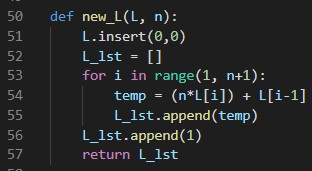
\includegraphics{new_L.jpg}
       \caption{Code Snippet: Pattern}
       \label{fig:my_label}
   \end{figure}
   And this code works really well to find for all values of $n$. 
   \begin{figure}[H]
       \centering
       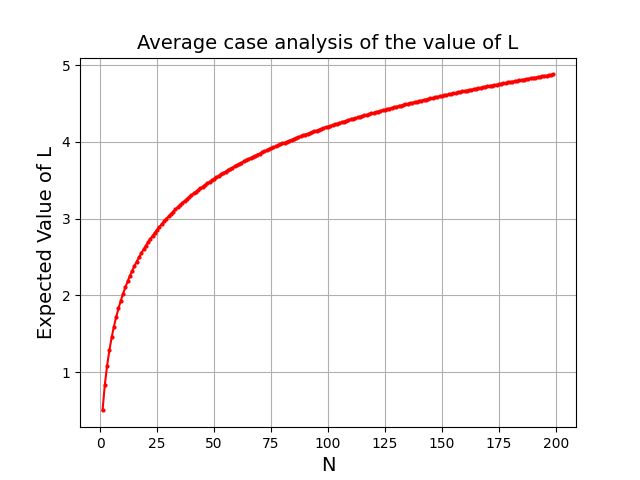
\includegraphics[width=10cm, height=10cm]{figure.png}
       \caption{For n values till 200}
       \label{fig:my_label}
   \end{figure}
  \end{mdframed}


\end{questions}
\end{document}

%%% Local Variables:
%%% mode: latex
%%% TeX-master: t
%%% End:
